\documentclass{article}
\usepackage[top=1.1in, bottom=1.5in, left=1in, right=1in]{geometry}
\usepackage{graphicx}
\usepackage[english]{babel}
\usepackage{enumitem}
\usepackage{pdfpages}
\usepackage{tabu}


\begin{document}
\title{Requirements Analysis Document (RAD) for 121Calendar}
\tableofcontents

\section{Introduction}
	\subsection{Purpose of the system}
	\subsection{Scope of the system}
	\subsection{Objectives and success citeria the project}
	\subsection{Definitions, acronyms and abbreveations}
	\subsection{References}
	\subsection{Overview}
\section{Current system}
\section{Proposed system}
	\subsection{Overview}
	\subsection{Functional Requirements}
	\subsection{Nonfunctional Requirements}
		\subsubsection{Usability}
		\subsubsection{Reliability}
		\subsubsection{Performance}
		\subsubsection{Supportability}
		\subsubsection{Implementation}
		\subsubsection{Interface}
		\subsubsection{Packaging}
		\subsubsection{Legal}
	\subsection{System models}
		\subsubsection{Scenarios}
			
				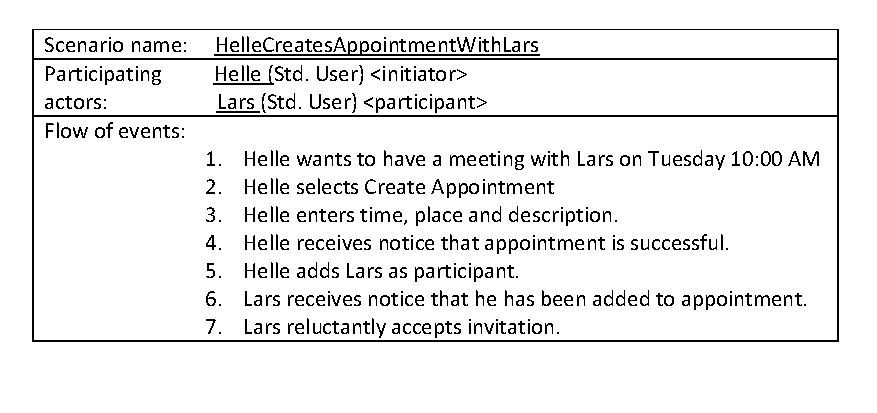
\includepdf[scale=0.8,pages=1,pagecommand=\paragraph{Scenario 1: Create Appointment:}]{docs/ScCreateApt.pdf}

			
				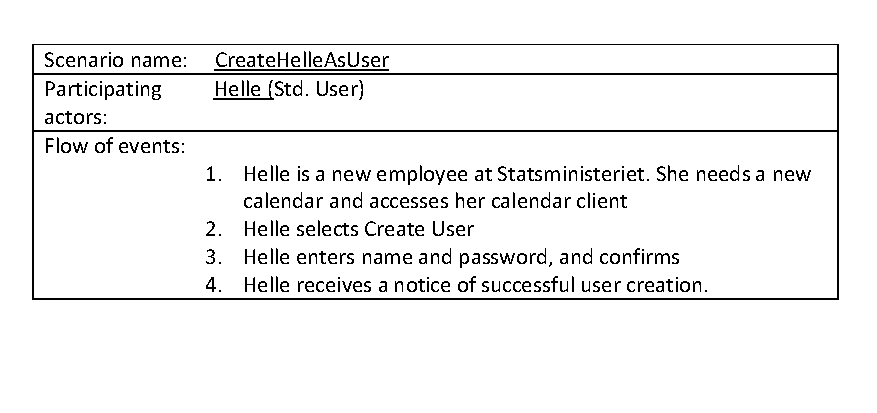
\includepdf[scale=0.8,pages=1,pagecommand=\paragraph{Scenario 2: Create User:}]{docs/ScCreateUser.pdf}
			
		\subsubsection{Use case model}
			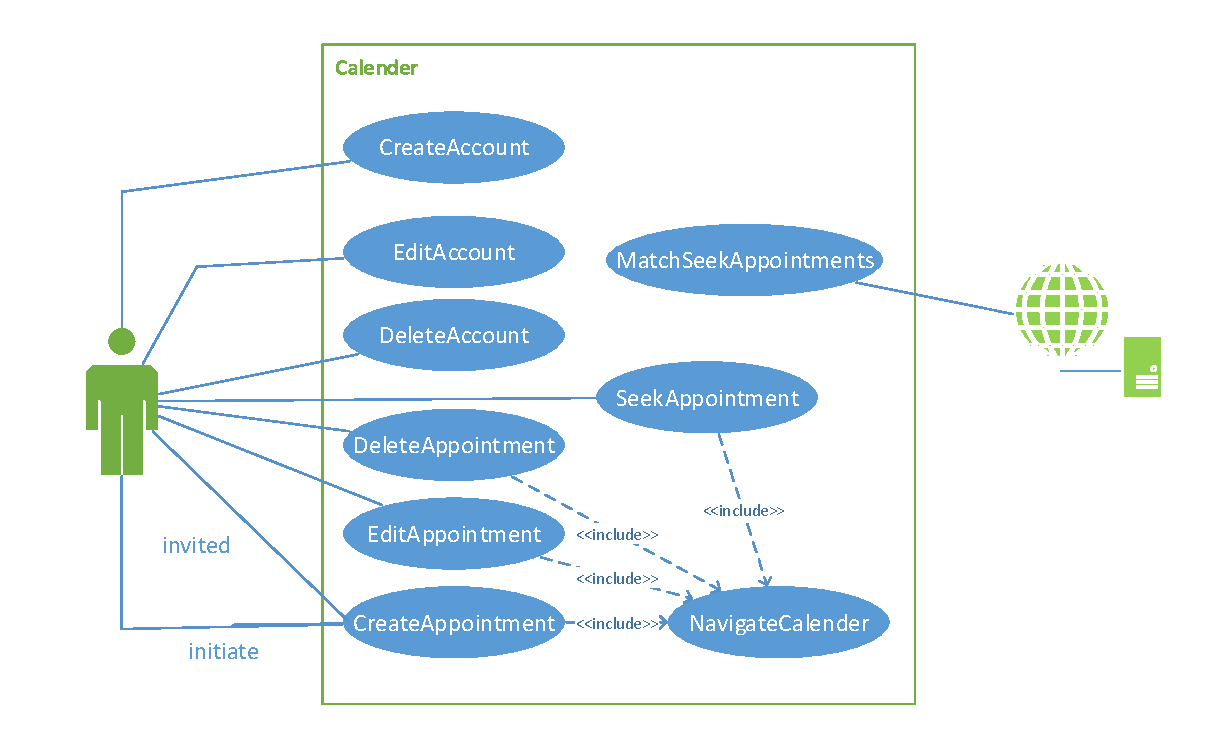
\includepdf{docs/UMLUsecaseDiagramCALENDAR.pdf}
		\subsubsection{Object model}
		\subsubsection{Dynamic model}
		\subsubsection{User interface}
\section{Glossary}

\end{document}
